\newpage
\section{Datasheet}
\vspace{1mm}
\Large \textbf{ADLQ - Line Following Robot Datasheet}

\begin{multicols}{2}

\subsection*{Product Overview}
\vspace{-2mm}
The ADLQ is a robot that follows black lines on a white background which has two modes. Mode One traverses a projected map whereas Mode Two finds the shortest path to a list of food pellets using A* algorithm. The modes can be changed using the onboard DIP switches. For optimal performance the robot’s operating voltage needs to be between 7.5 volts and 7.9 volts. ADLQ needs 6x1.2V batteries for operation.

\begin{figure}[H]
\centering
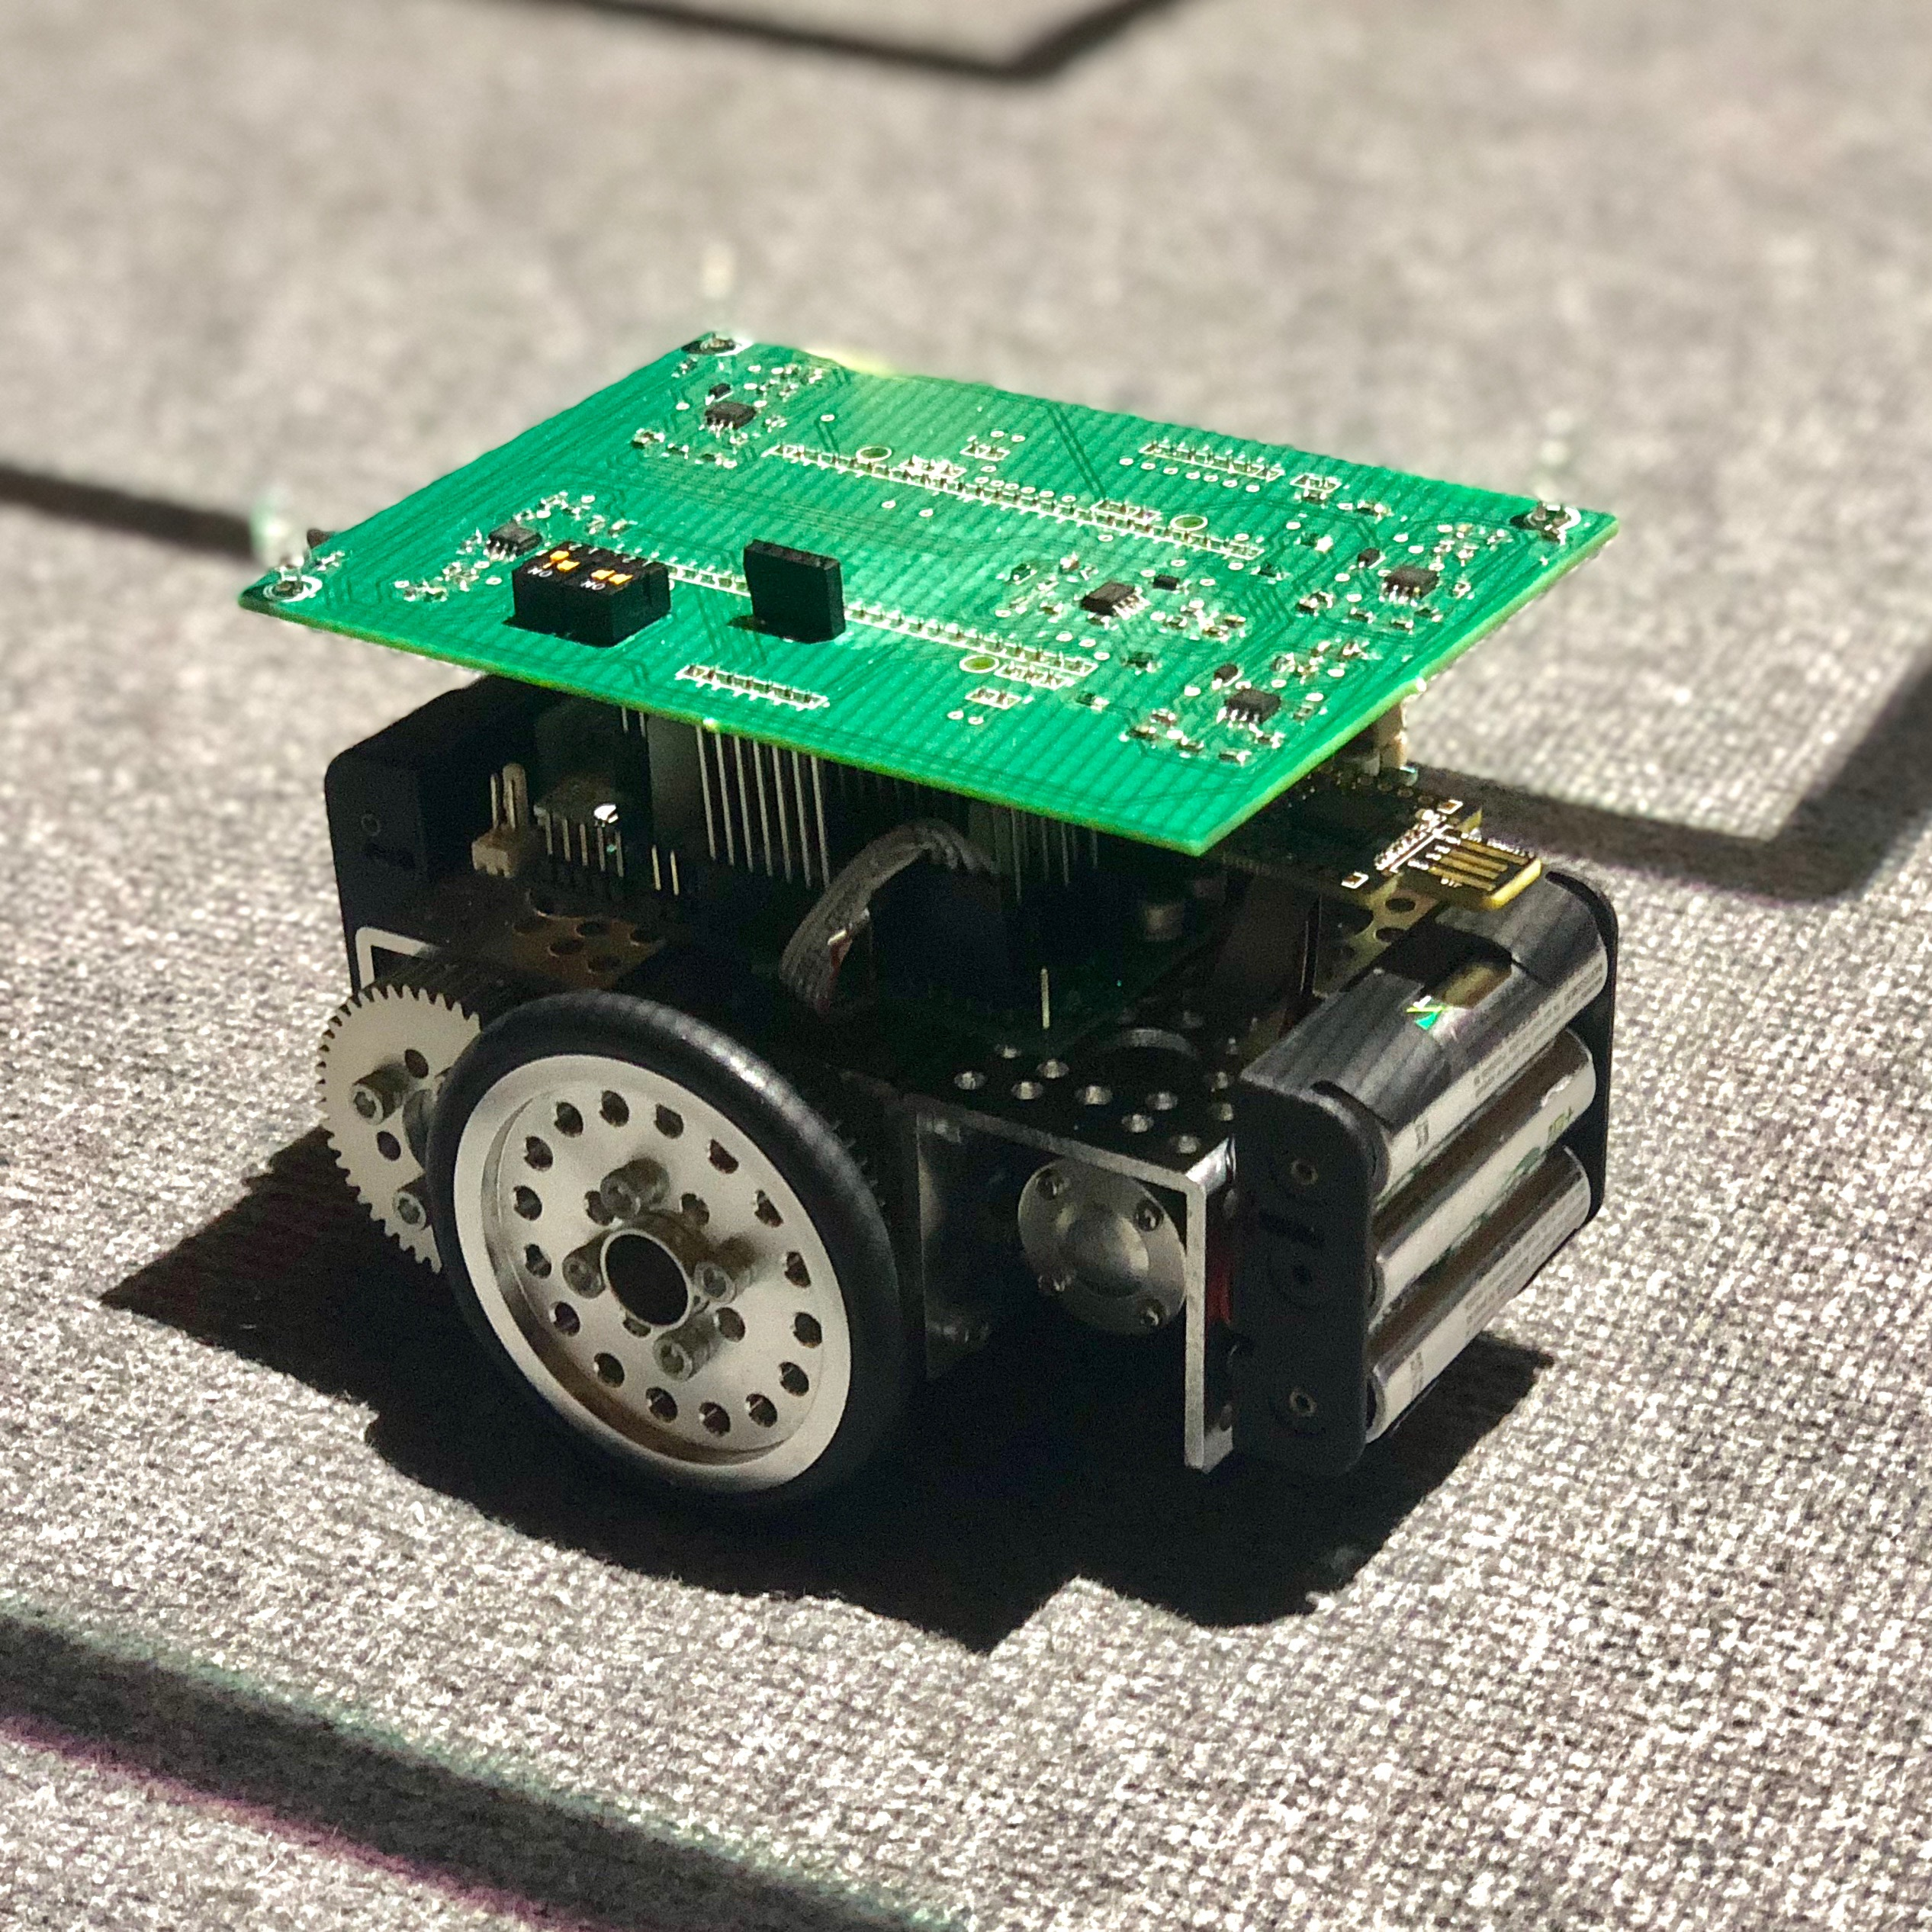
\includegraphics[width=0.4\textwidth]{figures/robot_img.JPG}
% \caption{BACK VIEW}
\end{figure}
\end{multicols}


\begin{multicols}{2}
\subsection*{Features}
\begin{itemize}
    \item 2 different modes:
    \begin{itemize}
        \item Traverse the map
        \item Shortest path
    \end{itemize}
    \item Travel Speed Range: 13-28cms\textsuperscript{-1}
\end{itemize}

\subsection*{Mode Selection}
The robot’s LEDs and mode configured using the onboard DIP switches. To enable the the LEDS, switch the left DIP switch 1 to ON. To enable the motors, switch the left DIP switch 2 to ON. For Mode 1 switch the right DIP switch 1 to ON and for Mode 2 switch the right DIP switch 1 to OFF.


\end{multicols}

\subsection*{Specifications}
\vspace{-4mm}
\begin{table}[h!]
\centering
\small
\resizebox{\textwidth}{!}{\begin{tabular}{|l|l|l|l|}
\hline
\textbf{PARAMETER} & \textbf{MIN} & \textbf{MAX} & \textbf{UNIT} \\ \hline
\textbf{\textit{Operating Voltage}} & 6.8 & 8.2 &   V                    \\ \hline
\textbf{\textit{Travel Speed}} & 13 & 28  & cms\textsuperscript{-1}      \\ \hline
\textbf{\textit{Line Detection Speed}} & 21 & 26 &   ms                   \\ \hline
\textbf{\textit{Wall Detection Speed}} & 14 & 19 &    ms                  \\ \hline
\textbf{\textit{Optimal Line Thickness}} & 18 & 22 &   mm                 \\ \hline
\textbf{\textit{Sensor Array Layout}} & \multicolumn{3}{l|}{2 left sensors, 2 right sensors and 1 centre sensor}             \\ \hline
\end{tabular}}
\end{table}

\subsection*{Robot Dimensions}
\vspace{-3mm}
\begin{figure}[H]
\centering
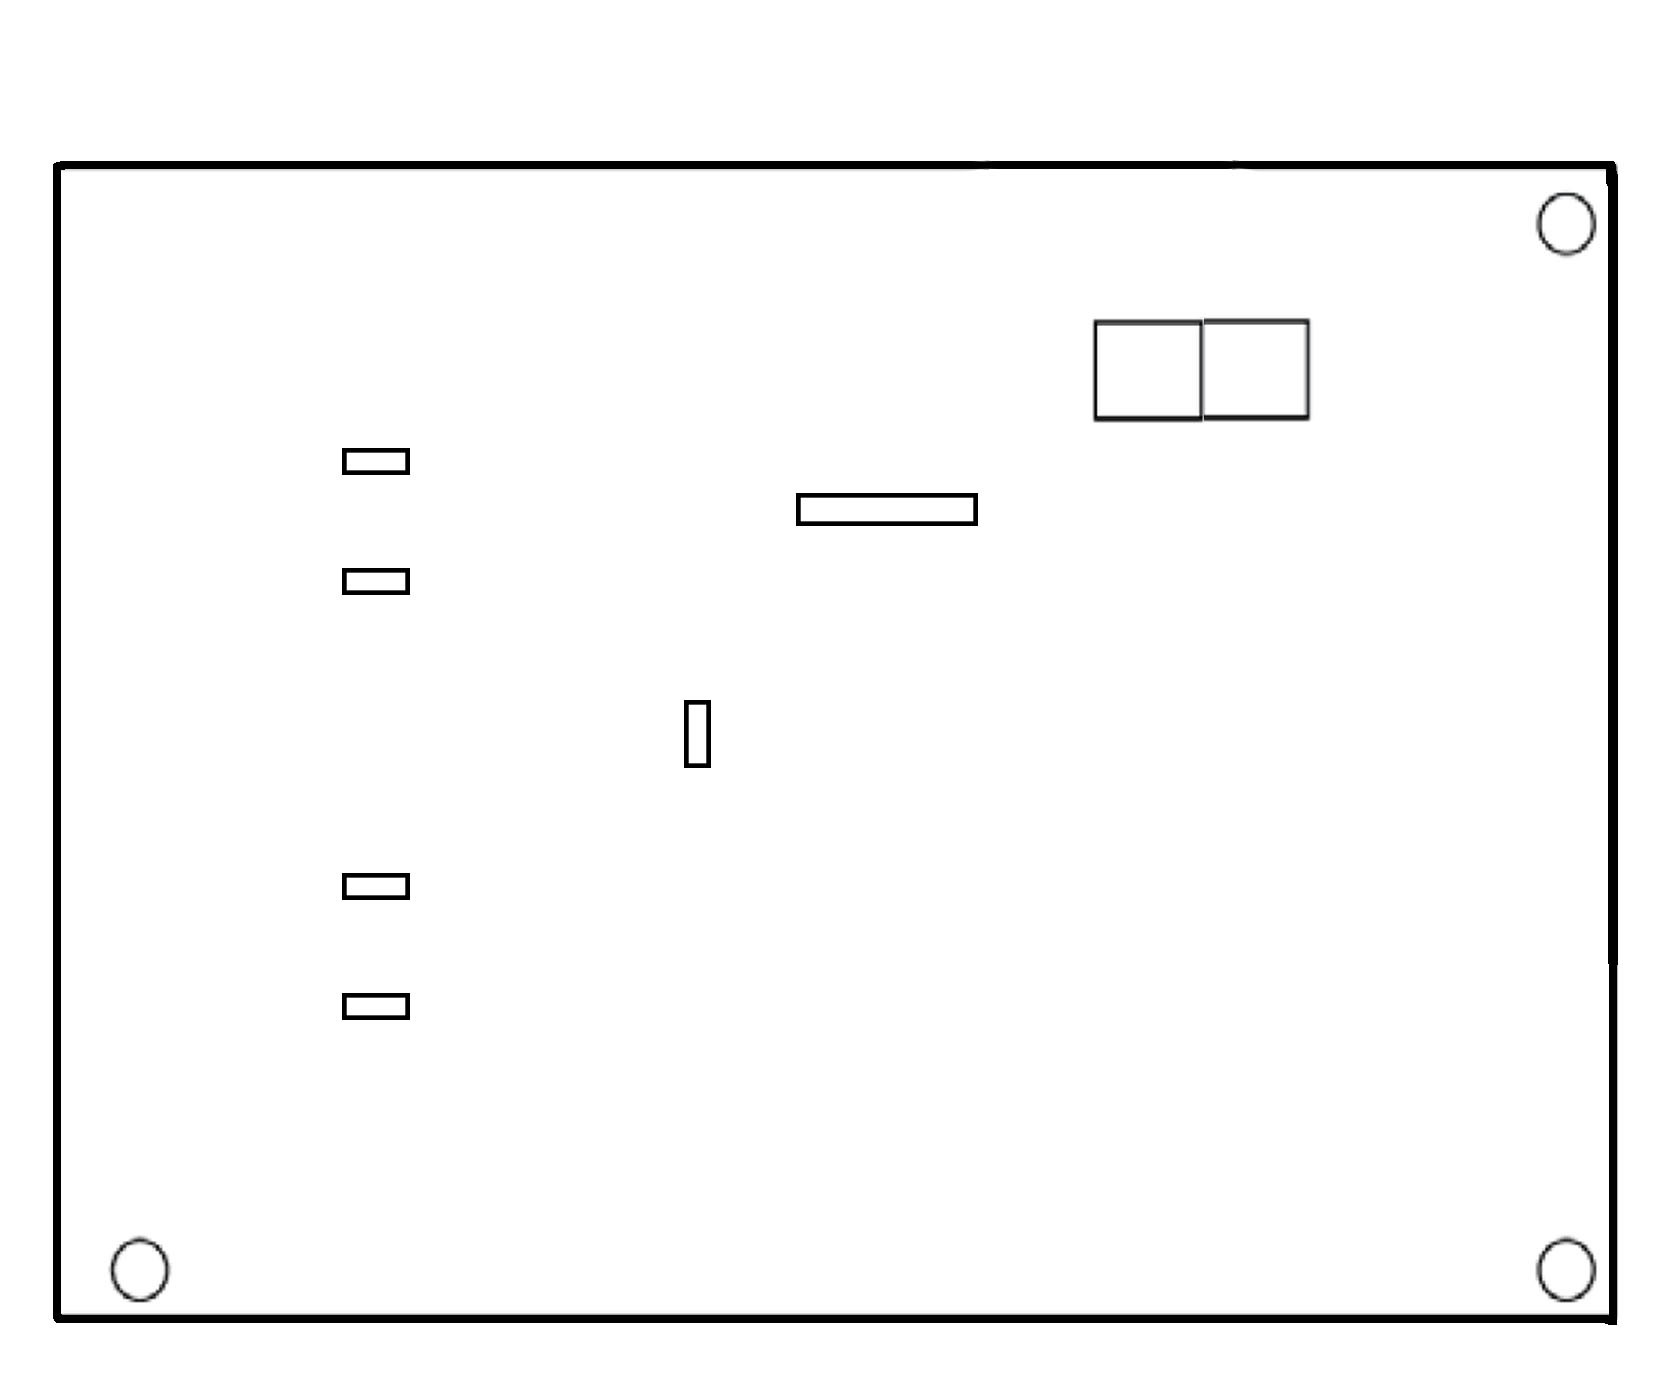
\includegraphics[width=0.39\textwidth]{figures/top_view.jpg}
\caption{TOP VIEW}
\end{figure}

\begin{figure}[H]
\centering
\hspace{-5mm}
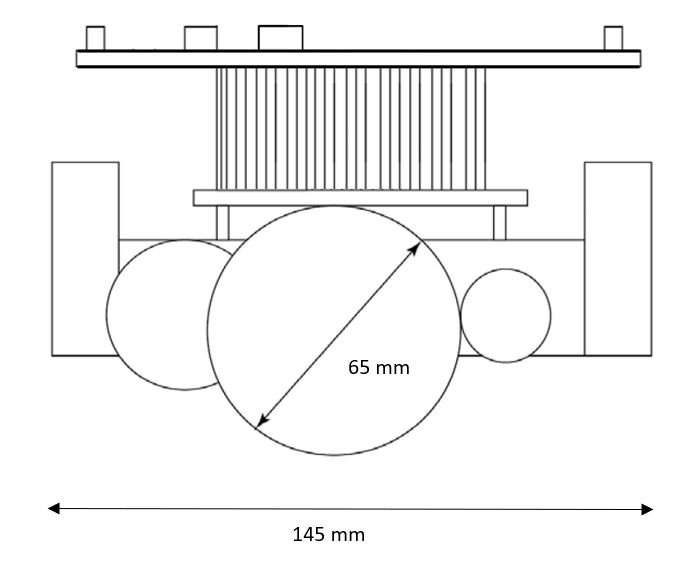
\includegraphics[width=0.45\textwidth]{figures/side_view.JPG}
\caption{SIDE VIEW}
\end{figure}

\begin{figure}[H]
\centering
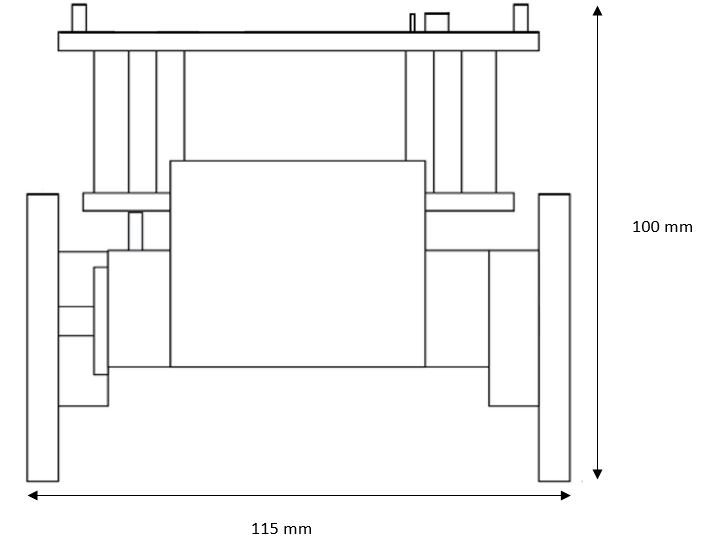
\includegraphics[width=0.42\textwidth]{figures/back_view.JPG}
\caption{BACK VIEW}
\end{figure}